% ============================================================
%  Reporte de Benchmark: MongoDB vs PostgreSQL JSONB
%  IT2iD - Universidad Politécnica de Chiapas
%  Bases de Datos en la Nube 2026
% ============================================================
\documentclass[12pt,a4paper]{article}

% --- Encoding & Language ---
\usepackage[utf8]{inputenc}
\usepackage[T1]{fontenc}
\usepackage[spanish,mexico]{babel}

% --- Layout ---
\usepackage[top=2.5cm, bottom=2.5cm, left=2.5cm, right=2.5cm]{geometry}
\usepackage{setspace}
\onehalfspacing

% --- Fonts ---
\usepackage{lmodern}
\usepackage{microtype}

% --- Graphics & Colors ---
\usepackage{graphicx}
\usepackage{xcolor}
\usepackage{float}
\usepackage{caption}
\usepackage{subcaption}

% --- Tables ---
\usepackage{booktabs}
\usepackage{tabularx}
\usepackage{longtable}
\usepackage{multirow}
\usepackage{array}
\usepackage{colortbl}

% --- Math ---
\usepackage{amsmath}
\usepackage{amssymb}

% --- Code listings ---
\usepackage{listings}
\usepackage{lstautogobble}

% --- Links & PDF metadata ---
\usepackage{hyperref}
\hypersetup{
    colorlinks=true,
    linkcolor=blue!60!black,
    urlcolor=blue!60!black,
    citecolor=green!50!black,
    pdftitle={Benchmark: MongoDB vs PostgreSQL JSONB bajo Contención de Recursos},
    pdfauthor={IT2iD - Universidad Politécnica de Chiapas},
    pdfsubject={Bases de Datos en la Nube 2026},
}

% --- Header / Footer ---
\usepackage{fancyhdr}
\pagestyle{fancy}
\fancyhf{}
\fancyhead[L]{\small\textit{Benchmark: MongoDB vs PostgreSQL JSONB}}
\fancyhead[R]{\small\textit{Bases de Datos en la Nube 2026}}
\fancyfoot[C]{\thepage}
\renewcommand{\headrulewidth}{0.4pt}

% --- Color palette ---
\definecolor{mongogreen}{HTML}{00684A}
\definecolor{pgblue}{HTML}{336791}
\definecolor{alertred}{HTML}{CC0000}
\definecolor{warnbg}{HTML}{FFF3CD}
\definecolor{okbg}{HTML}{D4EDDA}
\definecolor{errbg}{HTML}{F8D7DA}
\definecolor{codebg}{HTML}{F5F5F5}
\definecolor{headerbg}{HTML}{2C3E50}
\definecolor{headerfg}{HTML}{FFFFFF}

% --- Code style ---
\lstset{
  backgroundcolor=\color{codebg},
  basicstyle=\ttfamily\footnotesize,
  breaklines=true,
  breakatwhitespace=true,
  frame=single,
  rulecolor=\color{gray!40},
  numbers=left,
  numberstyle=\tiny\color{gray},
  numbersep=5pt,
  tabsize=2,
  showstringspaces=false,
  autogobble=true,
  captionpos=b,
}
\lstdefinelanguage{JavaScript}{
  keywords={function,var,let,const,return,if,else,for,while,true,false,null},
  keywordstyle=\color{blue!70!black}\bfseries,
  morestring=[b]",
  morestring=[b]',
  morecomment=[l]{//},
  morecomment=[s]{/*}{*/},
  stringstyle=\color{orange!80!black},
  commentstyle=\color{green!50!black}\itshape,
}
\lstdefinelanguage{SQL}{
  keywords={SELECT,FROM,WHERE,GROUP,BY,ORDER,LIMIT,SET,EXPLAIN,ANALYZE,BUFFERS,FORMAT,TEXT,ALTER,SYSTEM},
  keywordstyle=\color{blue!70!black}\bfseries,
  morestring=[b]',
  morecomment=[l]{--},
  stringstyle=\color{orange!80!black},
  commentstyle=\color{green!50!black}\itshape,
}

% --- Custom commands ---
\newcommand{\mongo}{\textcolor{mongogreen}{\textbf{MongoDB}}}
\newcommand{\pg}{\textcolor{pgblue}{\textbf{PostgreSQL JSONB}}}
\newcommand{\profileA}{\texttt{PROFILE\_A\_BASELINE}}
\newcommand{\profileB}{\texttt{PROFILE\_B\_MEDIUM}}
\newcommand{\profileC}{\texttt{PROFILE\_C\_SEVERE}}

\newcommand{\errorcell}[1]{\cellcolor{errbg}\textcolor{alertred}{\textbf{#1}}}
\newcommand{\okcell}[1]{\cellcolor{okbg}{#1}}
\newcommand{\warncell}[1]{\cellcolor{warnbg}{#1}}

% ============================================================
\begin{document}
% ============================================================

% ---- PORTADA -----------------------------------------------
\begin{titlepage}
  \centering
  \vspace*{1cm}

  {\Huge\bfseries\color{headerbg}
    Benchmark de Rendimiento\\[0.4em]
    \large\color{pgblue} MongoDB vs PostgreSQL JSONB\\
    \large\color{mongogreen} Bajo Contención de Recursos (cgroups v2)
  }

  \vspace{1.5cm}
  \rule{\linewidth}{0.5mm}
  \vspace{0.5cm}

  {\large
    \textbf{Asignatura:} Bases de Datos en la Nube 2026\\[0.3em]
    \textbf{Institución:} Universidad Politécnica de Chiapas\\[0.3em]
    \textbf{Programa:} IT2iD\\[0.3em]
    \textbf{Protocolo:} PDF §6 — Estricto\\[0.3em]
    \textbf{Dataset:} 500{,}000 registros sintéticos (órdenes de e-commerce)\\[0.3em]
    \textbf{Duración total de ejecución:} $\approx$ 10.52 horas
  }

  \vspace{1cm}
  \rule{\linewidth}{0.5mm}
  \vspace{1cm}

  \begin{tabular}{ll}
    \textbf{Motor A:}    & MongoDB 7.x (WiredTiger) \\
    \textbf{Motor B:}    & PostgreSQL 16 + JSONB \\
    \textbf{Orquestador:} & Docker Compose + cgroups v2 \\
    \textbf{Telemetría:} & cAdvisor + Node Exporter + Prometheus + Grafana \\
  \end{tabular}

  \vfill
  {\small Generado: \today}
\end{titlepage}

% ---- TABLA DE CONTENIDOS -----------------------------------
\tableofcontents
\newpage

% ============================================================
\section*{Agradecimientos}
\addcontentsline{toc}{section}{Agradecimientos}
% ============================================================

Deseo expresar un sincero y profundo agradecimiento a la \textbf{Universidad Politécnica de Chiapas (UPChiapas)} y al programa de \textbf{Ingeniería en Tecnologías de la Información e Innovación Digital (IT2iD)} por proveer la infraestructura académica, teórica y tecnológica fundamental que hizo posible el desarrollo riguroso de este trabajo de investigación experimental.

Un agradecimiento muy especial al \textbf{Catedrático y Docente de la asignatura Bases de Datos en la Nube (Edición 2026)}, por concebir y estructurar el protocolo experimental (\textit{Playbook de Métricas en Bases Documentales}), impulsando en nosotros los más altos estándares de rigor empírico, análisis a bajo nivel con subsistemas de Linux (cgroups v2, CFS throttling) y evaluación objetiva de motores de bases de datos bajo escenarios de alta contención en la nube.

Asimismo, extiendo mi agradecimiento a mis \textbf{compañeros de clase y colegas de laboratorio}, con quienes compartí valiosas discusiones técnicas en torno al aprovisionamiento y tuneo de contenedores Docker, gestión de volúmenes persistentes, mitigación de cuellos de botella de I/O en almacenamiento y estrategias de compactación de disco bajo sistemas virtualizados (WSL2/Hyper-V). Sus perspectivas, colaboración e intercambio de ideas enriquecieron significativamente la ejecución y el análisis de este proyecto.

\newpage


% ============================================================
\section{Especificaciones del Host y Entorno de Ejecución}
% ============================================================

\subsection{Hardware y Software del Host}

\begin{table}[H]
\centering
\caption{Especificaciones del entorno de ejecución}
\begin{tabular}{ll}
\toprule
\textbf{Componente}  & \textbf{Valor} \\
\midrule
Sistema Operativo    & Windows 11 (AMD64) \\
Python               & 3.14.0 \\
Motor Docker         & Docker Engine 29.9.2 \\
Driver MongoDB       & \texttt{pymongo} (nativo) \\
Driver PostgreSQL    & \texttt{psycopg} (nativo) \\
\bottomrule
\end{tabular}
\end{table}

\subsection{Perfiles de Recursos (cgroups v2)}

Cada perfil define un escenario de contención de recursos mediante límites de cgroups v2 aplicados a los contenedores Docker. Se ejecutaron tres perfiles progresivamente más restrictivos:

\begin{table}[H]
\centering
\caption{Perfiles de contención de recursos}
\begin{tabular}{llrrr}
\toprule
\textbf{ID} & \textbf{Nombre} & \textbf{CPUs} & \textbf{Memoria} & \textbf{mem\_swappiness} \\
\midrule
\rowcolor{okbg}
\profileA{} & Sin contención (Baseline)      & 4.0 & 4{,}096 MB & 0 \\
\rowcolor{warnbg}
\profileB{} & Contención media               & 2.0 & 2{,}048 MB & 0 \\
\rowcolor{errbg}
\profileC{} & Contención severa (throttling) & 1.0 & 1{,}024 MB & 0 \\
\bottomrule
\end{tabular}
\end{table}

\subsection{Stack de Telemetría}

\begin{itemize}
  \item \textbf{cAdvisor}: Métricas de contenedor (cgroups v2) — CPU throttling, RSS, límites
  \item \textbf{Node Exporter}: Métricas de host (I/O de disco, swap, red)
  \item \textbf{Prometheus}: \texttt{scrape\_interval = 1s} — recolección en tiempo real
  \item \textbf{Grafana}: Visualización de KPIs en dashboards durante la ejecución
\end{itemize}

% ============================================================
\section{Método de Medición y Verificación del Baseline}
% ============================================================

\subsection{Protocolo de Ejecución (PDF §6 — Estricto)}

El protocolo estricto del PDF §6 establece el siguiente ciclo por cada celda de medición:

\begin{enumerate}
  \item \textbf{Flush de caché}: \texttt{sync; echo 3 > /proc/sys/vm/drop\_caches}
  \item \textbf{Warmup}: 60 s (resultados descartados — solo para calentar JIT y cachés de BD)
  \item \textbf{Medición}: 300 s (5 minutos de medición activa)
  \item \textbf{Cooldown}: 60 s (ventilación térmica entre celdas)
\end{enumerate}

\subsection{Matriz de Mediciones}

\begin{table}[H]
\centering
\caption{Diseño factorial del benchmark}
\begin{tabular}{ll}
\toprule
\textbf{Dimensión}    & \textbf{Valores} \\
\midrule
Motores              & MongoDB, PostgreSQL JSONB \\
Perfiles             & A\_BASELINE, B\_MEDIUM, C\_SEVERE \\
Queries              & Q1 (Unwind + Group), Q2 (Sort + TopK) \\
Concurrencias        & 1, 10, 50 clientes simultáneos \\
Repeticiones         & 3 por celda \\
\midrule
\textbf{Total celdas} & $2 \times 3 \times 3 \times 3 \times 3 = \mathbf{162}$ ejecuciones \\
\bottomrule
\end{tabular}
\end{table}

\noindent\textbf{Nota:} Se midieron 3 variantes de query: \texttt{Q1}, \texttt{Q2\_disk\_false} y \texttt{Q2\_disk\_true}, lo que resulta en $2 \times 3 \times 3 \times 3 \times 3 = 162$ celdas totales.

\subsection{Queries Evaluadas}

\subsubsection{Q1 — Agregación con Unwind y Group By}

Simula un reporte de ingresos por país y categoría, expandiendo arreglos de ítems embebidos:

\begin{lstlisting}[language=JavaScript, caption={Q1 — MongoDB: Unwind + Group}]
db.orders.aggregate([
  { "$unwind": "$items" },
  { "$match": { "items.price": { "$gt": 50 } } },
  { "$group": {
      "_id": { "country": "$customer.geo.country",
                "category": "$items.category" },
      "total_revenue": { "$sum": { "$multiply": ["$items.qty",
                                                  "$items.price"] } },
      "avg_revenue":   { "$avg": { "$multiply": ["$items.qty",
                                                  "$items.price"] } },
      "count": { "$sum": 1 }
  }}
], { allowDiskUse: true })
\end{lstlisting}

\begin{lstlisting}[language=SQL, caption={Q1 — PostgreSQL JSONB: jsonb\_array\_elements + GROUP BY}]
SELECT data->'customer'->'geo'->>'country' AS country,
       item->>'category'                   AS category,
       SUM((item->>'qty')::numeric * (item->>'price')::numeric)
           AS total_revenue,
       AVG((item->>'qty')::numeric * (item->>'price')::numeric)
           AS avg_revenue,
       COUNT(*) AS count
FROM orders, jsonb_array_elements(data->'items') AS item
WHERE (item->>'price')::numeric > 50
GROUP BY 1, 2;
\end{lstlisting}

\subsubsection{Q2 — Ordenamiento TopK (Sort + Limit)}

Recupera las 1{,}000 órdenes con mayor total de pago entre órdenes completadas desde enero 2026:

\begin{lstlisting}[language=JavaScript, caption={Q2 — MongoDB: Sort + Limit + Project}]
db.orders.aggregate([
  { "$match": { "payment.status": "completed",
                "timestamp": { "$gte": "2026-01-01T00:00:00Z" } } },
  { "$sort":  { "payment.final_total": -1 } },
  { "$limit": 1000 },
  { "$project": { "order_id": 1, "customer.id": 1,
                   "payment.final_total": 1 } }
], { allowDiskUse: true })
\end{lstlisting}

\begin{lstlisting}[language=SQL, caption={Q2 — PostgreSQL JSONB: Sort + Limit}]
SELECT data->>'order_id'                          AS order_id,
       data->'customer'->>'id'                    AS customer_id,
       (data->'payment'->>'final_total')::numeric AS final_total
FROM orders
WHERE data->'payment'->>'status' = 'completed'
  AND (data->>'timestamp') >= '2026-01-01T00:00:00Z'
ORDER BY final_total DESC
LIMIT 1000;
\end{lstlisting}

\subsection{Verificación del Baseline}

En \profileA{} (4 CPUs, 4 GB RAM) se verificó que:
\begin{itemize}
  \item \texttt{container\_cpu\_cfs\_throttled\_seconds\_total} $\approx 0$ durante el warmup
  \item Ambos motores responden correctamente antes de iniciar la medición
  \item Los volúmenes Docker (\texttt{mongo\_data}, \texttt{pg\_data}) persisten datos entre reinicios de contenedor
\end{itemize}

% ============================================================
\section{Resultados Consolidados}
% ============================================================

Las siguientes tablas presentan el promedio de las 3 repeticiones por celda (motor, perfil, query, concurrencia).

\subsection{MongoDB — Resultados por Perfil}

\begin{longtable}{lllrrrrrr}
\caption{Resultados MongoDB (promedio de 3 repeticiones)} \label{tab:mongodb} \\
\toprule
\textbf{Perfil} & \textbf{Query} & \textbf{C} & \textbf{QPS} & \textbf{P50 ms} & \textbf{P95 ms} & \textbf{P99 ms} & \textbf{Thr. s} & \textbf{RSS MB} \\
\midrule
\endfirsthead
\multicolumn{9}{c}{\tablename\ \thetable{} -- continuación} \\
\toprule
\textbf{Perfil} & \textbf{Query} & \textbf{C} & \textbf{QPS} & \textbf{P50 ms} & \textbf{P95 ms} & \textbf{P99 ms} & \textbf{Thr. s} & \textbf{RSS MB} \\
\midrule
\endhead
\bottomrule
\endfoot
% PROFILE_A_BASELINE
\rowcolor{gray!8}
A\_BASE & Q1            & 1  & 0.70 & 1{,}420   & 1{,}555   & 1{,}715   & 0.00     & 664 \\
\rowcolor{gray!8}
A\_BASE & Q1            & 10 & 0.66 & 15{,}360  & 16{,}485  & 16{,}724  & 1{,}824  & 735 \\
\rowcolor{gray!8}
A\_BASE & Q1            & 50 & 0.34 & 144{,}004 & 157{,}906 & 163{,}595 & 3{,}193  & 899 \\
A\_BASE & Q2\_disk\_off & 1  & 1.78 & 533       & 769       & 857       & 0.00     & 838 \\
A\_BASE & Q2\_disk\_off & 10 & 2.54 & 4{,}068   & 4{,}694   & 4{,}837   & 1{,}791  & 813 \\
A\_BASE & Q2\_disk\_off & 50 & 2.22 & 22{,}855  & 29{,}821  & 33{,}551  & 2{,}435  & 826 \\
A\_BASE & Q2\_disk\_on  & 1  & 1.79 & 555       & 626       & 690       & 0.00     & 825 \\
A\_BASE & Q2\_disk\_on  & 10 & 2.39 & 4{,}187   & 5{,}030   & 8{,}930   & 1{,}792  & 820 \\
A\_BASE & Q2\_disk\_on  & 50 & 2.09 & 23{,}761  & 33{,}360  & 38{,}655  & 2{,}433  & 829 \\
\midrule
% PROFILE_B_MEDIUM
\rowcolor{warnbg}
B\_MED  & Q1            & 1  & 0.19 & 5{,}348    & 10{,}649  & 12{,}486  & 3.93    & 676 \\
\rowcolor{warnbg}
B\_MED  & Q1            & 10 & 0.22 & 42{,}954   & 65{,}566  & 65{,}593  & 1{,}279 & 670 \\
\rowcolor{errbg}
B\_MED  & Q1            & 50 & 0.03 & 1{,}497{,}361 & 1{,}601{,}480 & 1{,}637{,}976 & 16{,}318 & 1{,}076 \\
\rowcolor{warnbg}
B\_MED  & Q2\_disk\_off & 1  & 0.06 & 44{,}368   & 59{,}567  & 73{,}511  & 107     & 944 \\
\rowcolor{warnbg}
B\_MED  & Q2\_disk\_off & 10 & 0.08 & 206{,}337  & 254{,}872 & 254{,}877 & 2{,}162 & 852 \\
\rowcolor{warnbg}
B\_MED  & Q2\_disk\_off & 50 & 0.73 & 300{,}972  & 324{,}023 & 326{,}581 & 4{,}072 & 806 \\
\rowcolor{warnbg}
B\_MED  & Q2\_disk\_on  & 1  & 0.46 & 2{,}149    & 2{,}322   & 2{,}445   & 0.00    & 696 \\
\rowcolor{warnbg}
B\_MED  & Q2\_disk\_on  & 10 & 0.70 & 14{,}502   & 16{,}793  & 17{,}375  & 1{,}944 & 677 \\
\rowcolor{warnbg}
B\_MED  & Q2\_disk\_on  & 50 & 1.19 & 42{,}836   & 65{,}132  & 66{,}857  & 3{,}078 & 764 \\
\midrule
% PROFILE_C_SEVERE
\rowcolor{errbg}
C\_SEV  & Q1            & 1  & 0.59 & 1{,}676    & 1{,}752   & 1{,}799   & 8.26    & 448 \\
\rowcolor{errbg}
C\_SEV  & Q1            & 10 & 0.24 & 41{,}431   & 43{,}533  & 44{,}483  & 3{,}038 & 466 \\
\rowcolor{errbg}
C\_SEV  & Q1            & 50 & 0.22 & 229{,}801  & 232{,}696 & 234{,}034 & 4{,}872 & 603 \\
\rowcolor{errbg}
C\_SEV  & Q2\_disk\_off & 1  & 0.20 & 5{,}101    & 5{,}240   & 5{,}317   & 10.80   & 572 \\
\rowcolor{errbg}
C\_SEV  & Q2\_disk\_off & 10 & 0.16 & 62{,}949   & 65{,}484  & 65{,}517  & 2{,}298 & 512 \\
\rowcolor{errbg}
C\_SEV  & Q2\_disk\_off & 50 & 0.43 & 116{,}211  & 120{,}126 & 120{,}199 & 3{,}322 & 559 \\
\rowcolor{errbg}
C\_SEV  & Q2\_disk\_on  & 1  & 0.20 & 5{,}110    & 5{,}230   & 5{,}405   & 11.07   & 521 \\
\rowcolor{errbg}
C\_SEV  & Q2\_disk\_on  & 10 & 0.16 & 61{,}162   & 64{,}835  & 64{,}873  & 2{,}210 & 505 \\
\rowcolor{errbg}
C\_SEV  & Q2\_disk\_on  & 50 & 0.42 & 118{,}378  & 124{,}037 & 125{,}916 & 3{,}421 & 572 \\
\end{longtable}

\subsection{PostgreSQL JSONB — Resultados por Perfil}

\begin{longtable}{lllrrrrrll}
\caption{Resultados PostgreSQL JSONB (promedio de 3 repeticiones)} \label{tab:postgresql} \\
\toprule
\textbf{Perfil} & \textbf{Query} & \textbf{C} & \textbf{QPS} & \textbf{P50 ms} & \textbf{P95 ms} & \textbf{P99 ms} & \textbf{Thr. s} & \textbf{Spill} & \textbf{Status} \\
\midrule
\endfirsthead
\multicolumn{10}{c}{\tablename\ \thetable{} -- continuación} \\
\toprule
\textbf{Perfil} & \textbf{Query} & \textbf{C} & \textbf{QPS} & \textbf{P50 ms} & \textbf{P95 ms} & \textbf{P99 ms} & \textbf{Thr. s} & \textbf{Spill} & \textbf{Status} \\
\midrule
\endhead
\bottomrule
\endfoot
% PROFILE_A_BASELINE
\rowcolor{gray!8}
A\_BASE & Q1            & 1  & 0.12 & 8{,}133    & 12{,}124  & 14{,}111  & 62.00   & No  & \textcolor{green!60!black}{ok} \\
\rowcolor{gray!8}
A\_BASE & Q1            & 10 & 0.05 & 203{,}309  & 281{,}293 & 281{,}653 & 2{,}210 & No  & \textcolor{green!60!black}{ok} \\
\rowcolor{errbg}
A\_BASE & Q1            & 50 & 0.00 & ---        & ---       & ---       & 0.00    & No  & \textcolor{alertred}{\textbf{error}} \\
A\_BASE & Q2\_disk\_off & 1  & 4.32 & 196        & 533       & 959       & 0.00    & \textcolor{alertred}{Sí} & \textcolor{green!60!black}{ok} \\
A\_BASE & Q2\_disk\_off & 10 & 1.63 & 5{,}492    & 11{,}812  & 13{,}541  & 0.00    & \textcolor{alertred}{Sí} & \textcolor{green!60!black}{ok} \\
A\_BASE & Q2\_disk\_off & 50 & 1.28 & 41{,}227   & 63{,}944  & 73{,}150  & 0.00    & \textcolor{alertred}{Sí} & \textcolor{green!60!black}{ok} \\
A\_BASE & Q2\_disk\_on  & 1  & 3.32 & 207        & 1{,}036   & 1{,}477   & 0.00    & No  & \textcolor{green!60!black}{ok} \\
A\_BASE & Q2\_disk\_on  & 10 & 1.30 & 6{,}519    & 14{,}686  & 17{,}395  & 0.00    & No  & \textcolor{green!60!black}{ok} \\
A\_BASE & Q2\_disk\_on  & 50 & 0.86 & 60{,}173   & 107{,}056 & 128{,}758 & 0.00    & No  & \textcolor{green!60!black}{ok} \\
\midrule
% PROFILE_B_MEDIUM
\rowcolor{warnbg}
B\_MED  & Q1            & 1  & 0.29 & 3{,}354    & 4{,}655   & 5{,}681   & 131     & No  & \textcolor{green!60!black}{ok} \\
\rowcolor{warnbg}
B\_MED  & Q1            & 10 & 0.15 & 67{,}084   & 71{,}992  & 72{,}770  & 2{,}467 & No  & \textcolor{green!60!black}{ok} \\
\rowcolor{errbg}
B\_MED  & Q1            & 50 & 0.00 & ---        & ---       & ---       & 2{,}562 & No  & \textcolor{alertred}{\textbf{error}} \\
\rowcolor{warnbg}
B\_MED  & Q2\_disk\_off & 1  & 2.37 & 411        & 523       & 586       & 609     & \textcolor{alertred}{Sí} & \textcolor{green!60!black}{ok} \\
\rowcolor{warnbg}
B\_MED  & Q2\_disk\_off & 10 & 1.30 & 5{,}836    & 13{,}226  & 13{,}866  & 2{,}176 & \textcolor{alertred}{Sí} & \textcolor{green!60!black}{ok} \\
\rowcolor{warnbg}
B\_MED  & Q2\_disk\_off & 50 & 1.22 & 45{,}417   & 51{,}978  & 58{,}461  & 2{,}676 & \textcolor{alertred}{Sí} & \textcolor{green!60!black}{ok} \\
\rowcolor{warnbg}
B\_MED  & Q2\_disk\_on  & 1  & 2.09 & 486        & 612       & 687       & 627     & No  & \textcolor{green!60!black}{ok} \\
\rowcolor{warnbg}
B\_MED  & Q2\_disk\_on  & 10 & 1.21 & 6{,}530    & 13{,}561  & 14{,}001  & 2{,}182 & No  & \textcolor{green!60!black}{ok} \\
\rowcolor{warnbg}
B\_MED  & Q2\_disk\_on  & 50 & 1.20 & 45{,}862   & 52{,}493  & 56{,}482  & 2{,}716 & No  & \textcolor{green!60!black}{ok} \\
\midrule
% PROFILE_C_SEVERE
\rowcolor{errbg}
C\_SEV  & Q1            & 1  & 0.16 & 6{,}218    & 6{,}633   & 6{,}698   & 457     & No  & \textcolor{green!60!black}{ok} \\
\rowcolor{errbg}
C\_SEV  & Q1            & 10 & 0.77 & 178{,}496  & 243{,}832 & 243{,}832 & 2{,}945 & No  & \textcolor{alertred}{\textbf{error}} \\
\rowcolor{errbg}
C\_SEV  & Q1            & 50 & 0.00 & ---        & ---       & ---       & 3{,}162 & No  & \textcolor{alertred}{\textbf{error}} \\
C\_SEV  & Q2\_disk\_off & 1  & 0.97 & 1{,}012    & 1{,}208   & 1{,}298   & 943     & \textcolor{alertred}{Sí} & \textcolor{green!60!black}{ok} \\
C\_SEV  & Q2\_disk\_off & 10 & 0.63 & 10{,}642   & 25{,}996  & 27{,}062  & 2{,}528 & \textcolor{alertred}{Sí} & \textcolor{green!60!black}{ok} \\
C\_SEV  & Q2\_disk\_off & 50 & 0.55 & 95{,}688   & 128{,}459 & 141{,}595 & 3{,}091 & \textcolor{alertred}{Sí} & \textcolor{green!60!black}{ok} \\
C\_SEV  & Q2\_disk\_on  & 1  & 0.96 & 1{,}036    & 1{,}214   & 1{,}306   & 941     & No  & \textcolor{green!60!black}{ok} \\
C\_SEV  & Q2\_disk\_on  & 10 & 0.63 & 11{,}570   & 26{,}097  & 26{,}951  & 2{,}519 & No  & \textcolor{green!60!black}{ok} \\
C\_SEV  & Q2\_disk\_on  & 50 & 0.55 & 93{,}220   & 126{,}142 & 137{,}162 & 3{,}122 & No  & \textcolor{green!60!black}{ok} \\
\end{longtable}

% ============================================================
\section{Análisis Gráfico}
% ============================================================

\subsection{Latencia P99 vs Concurrencia — Q1 (Unwind + Group)}

\begin{figure}[H]
  \centering
  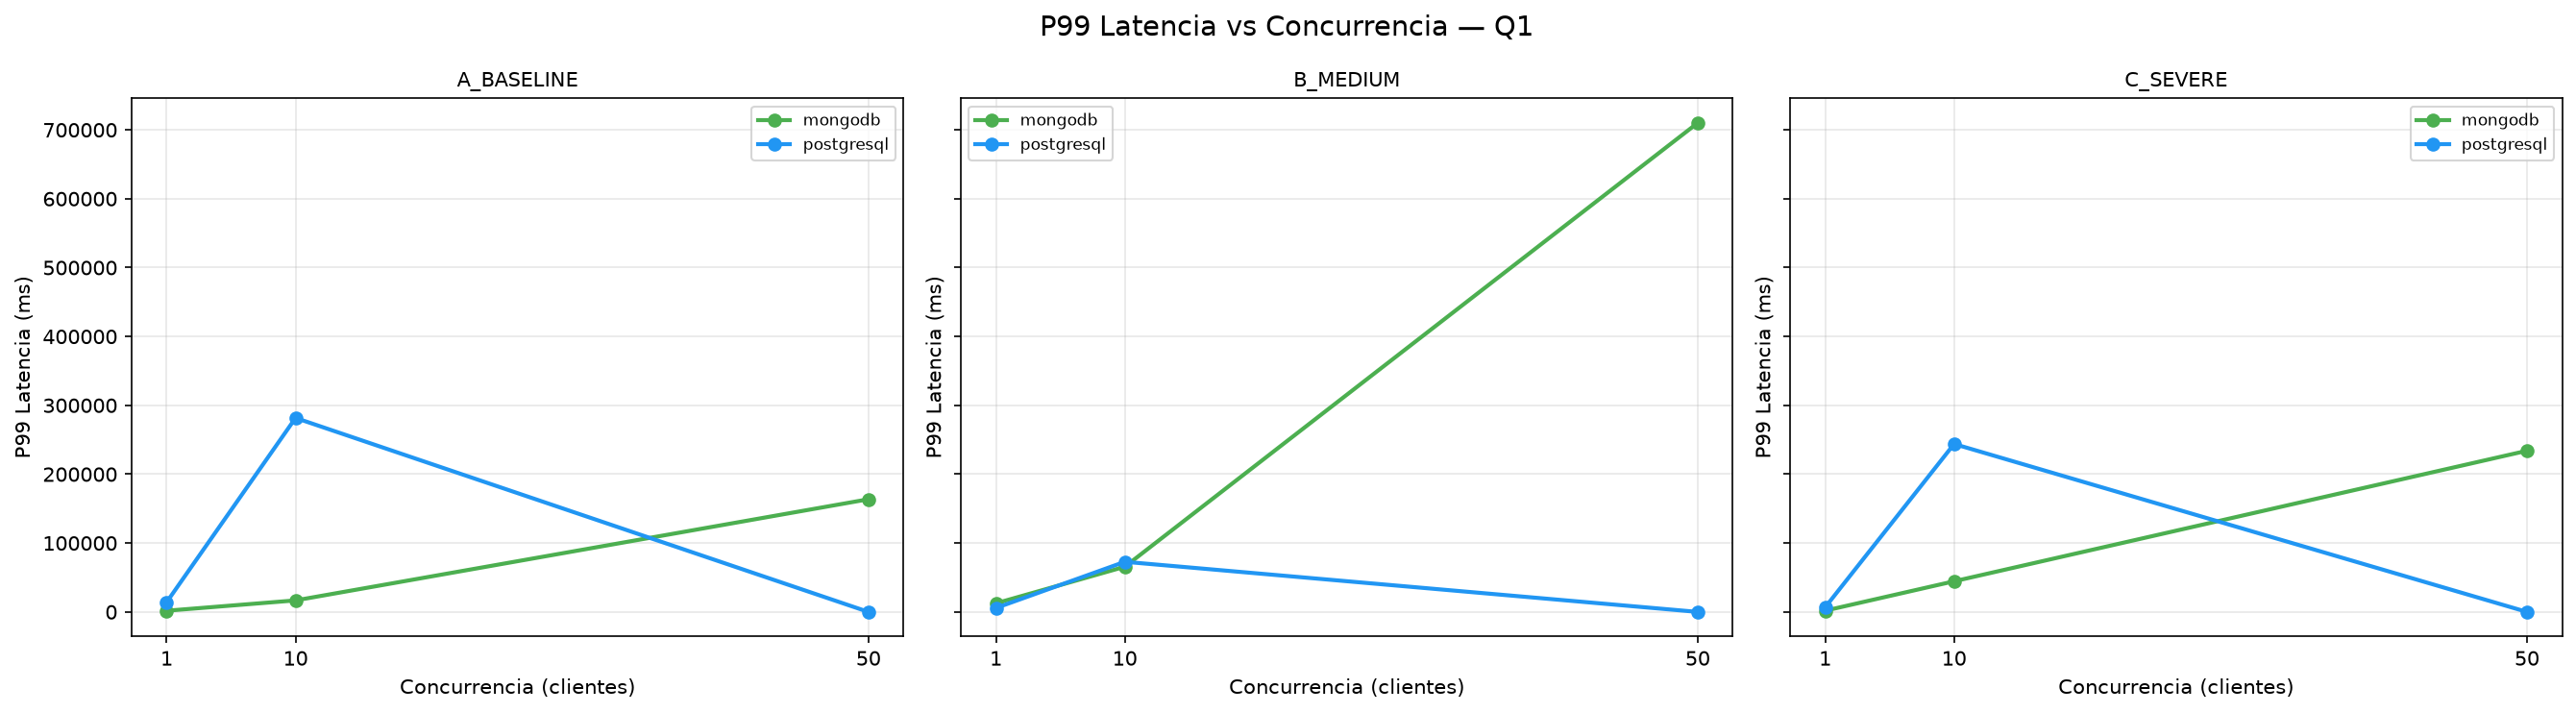
\includegraphics[width=0.92\textwidth]{graphs/p99_vs_concurrency_Q1.png}
  \caption{Latencia P99 en función de la concurrencia para Q1. Se observa que \pg{} colapsa (error/OOM) a C=50 en todos los perfiles, mientras que \mongo{} mantiene una degradación gradual.}
  \label{fig:p99_q1}
\end{figure}

\subsection{Latencia P99 vs Concurrencia — Q2 sin Volcado a Disco}

\begin{figure}[H]
  \centering
  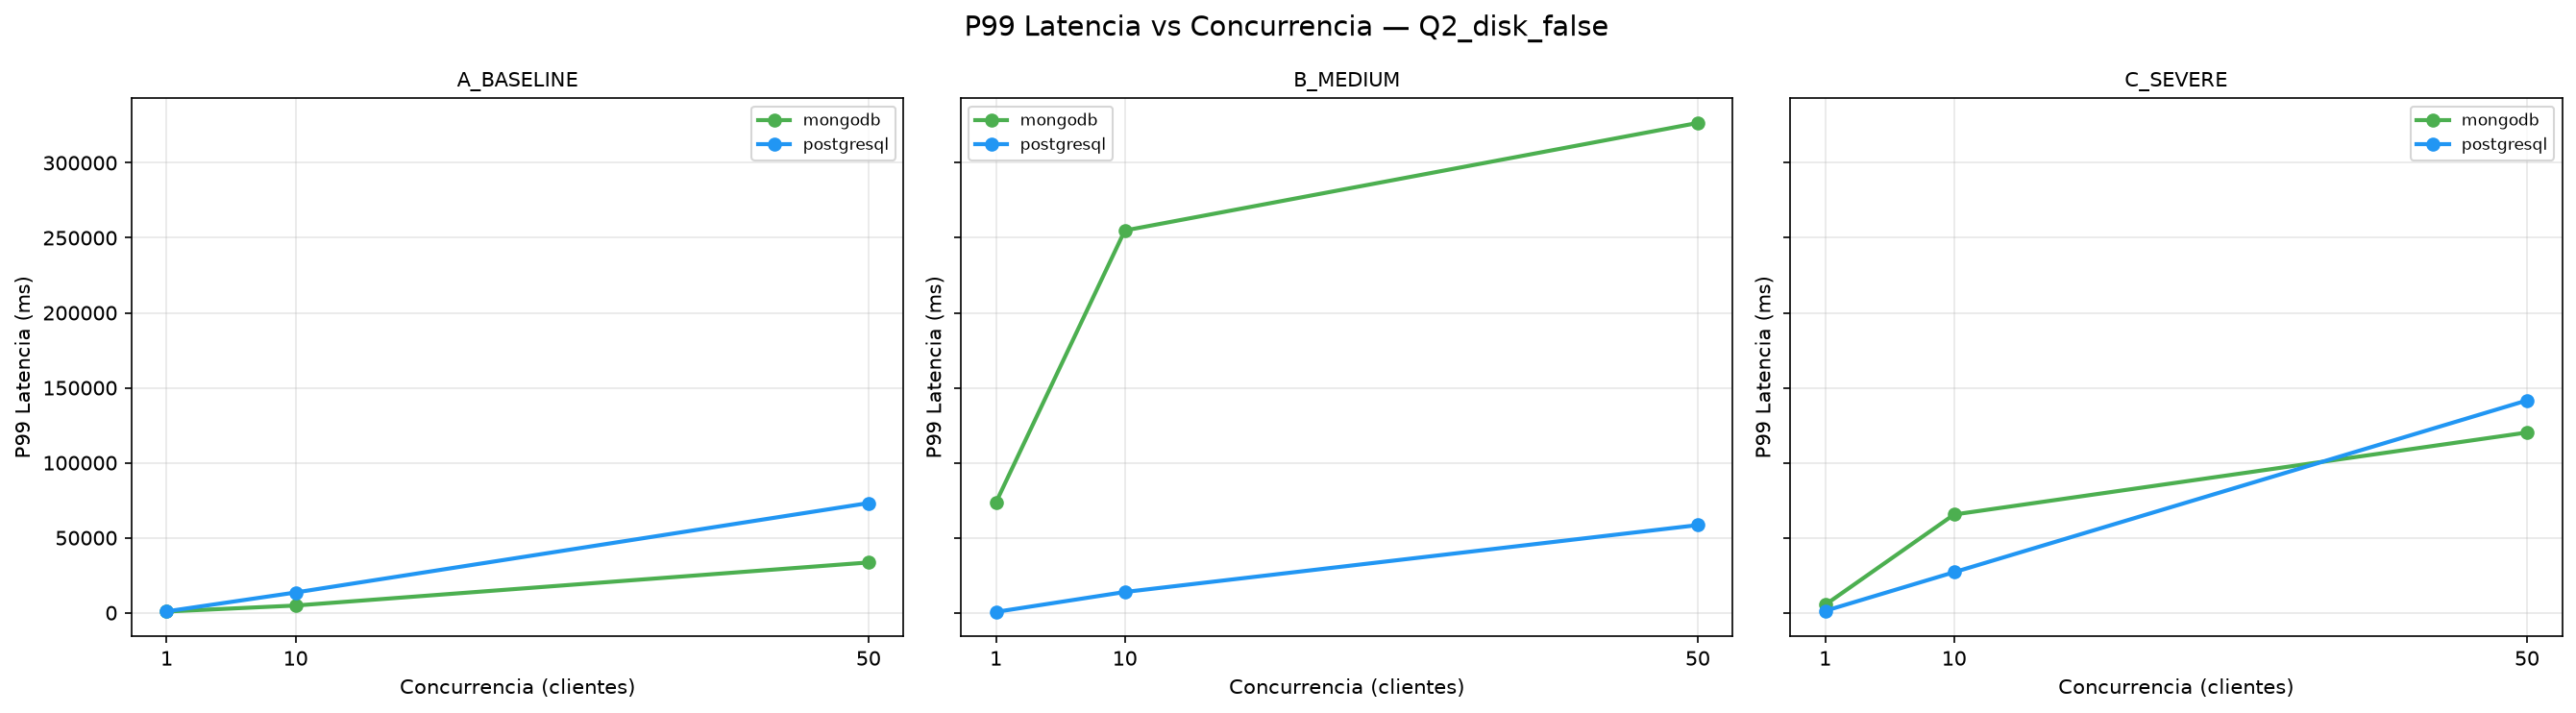
\includegraphics[width=0.92\textwidth]{graphs/p99_vs_concurrency_Q2_disk_false.png}
  \caption{Latencia P99 para Q2 con \texttt{work\_mem=4MB} (Q2\_disk\_false). PostgreSQL presenta \texttt{disk\_spill=True} en todos los perfiles bajo esta configuración, elevando su latencia.}
  \label{fig:p99_q2_false}
\end{figure}

\subsection{Latencia P99 vs Concurrencia — Q2 con Volcado a Disco Habilitado}

\begin{figure}[H]
  \centering
  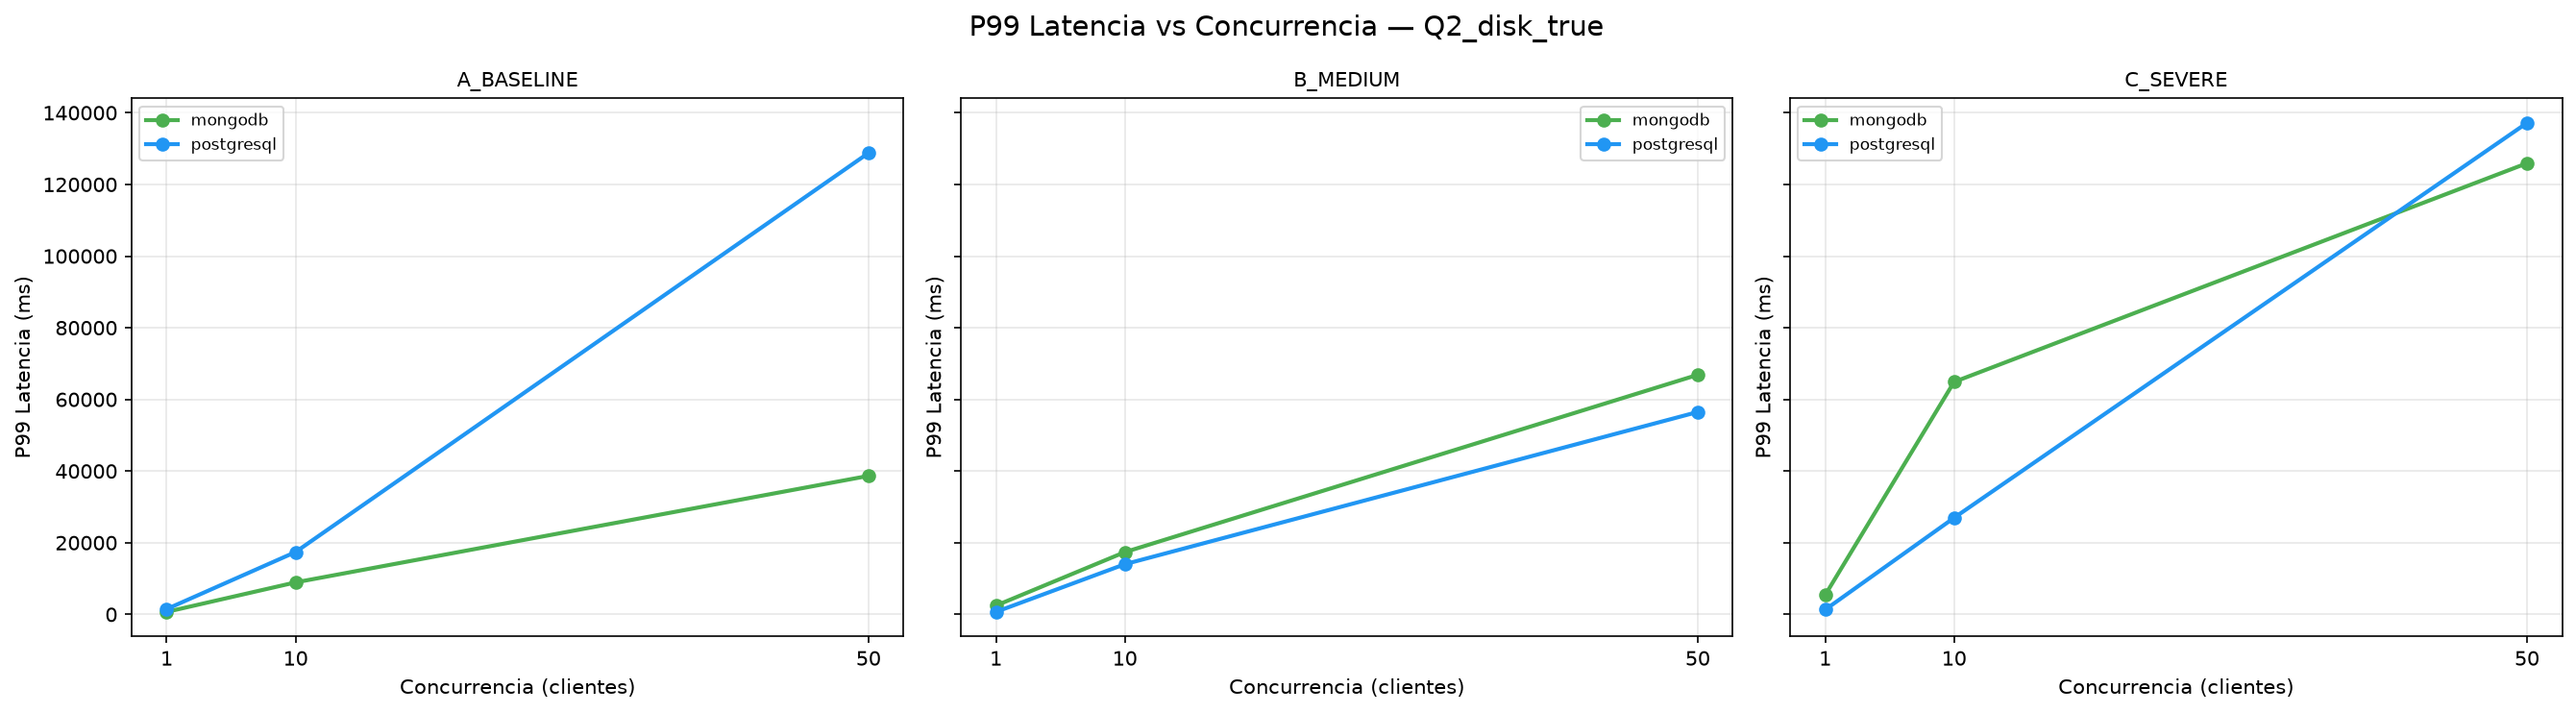
\includegraphics[width=0.92\textwidth]{graphs/p99_vs_concurrency_Q2_disk_true.png}
  \caption{Latencia P99 para Q2 con \texttt{work\_mem=64MB} (Q2\_disk\_true). Con memoria suficiente, PostgreSQL elimina los bloques \textit{lossy} y reduce la latencia en un factor de $\approx 5.1\times$.}
  \label{fig:p99_q2_true}
\end{figure}

\subsection{CPU Throttling Acumulado vs QPS}

\begin{figure}[H]
  \centering
  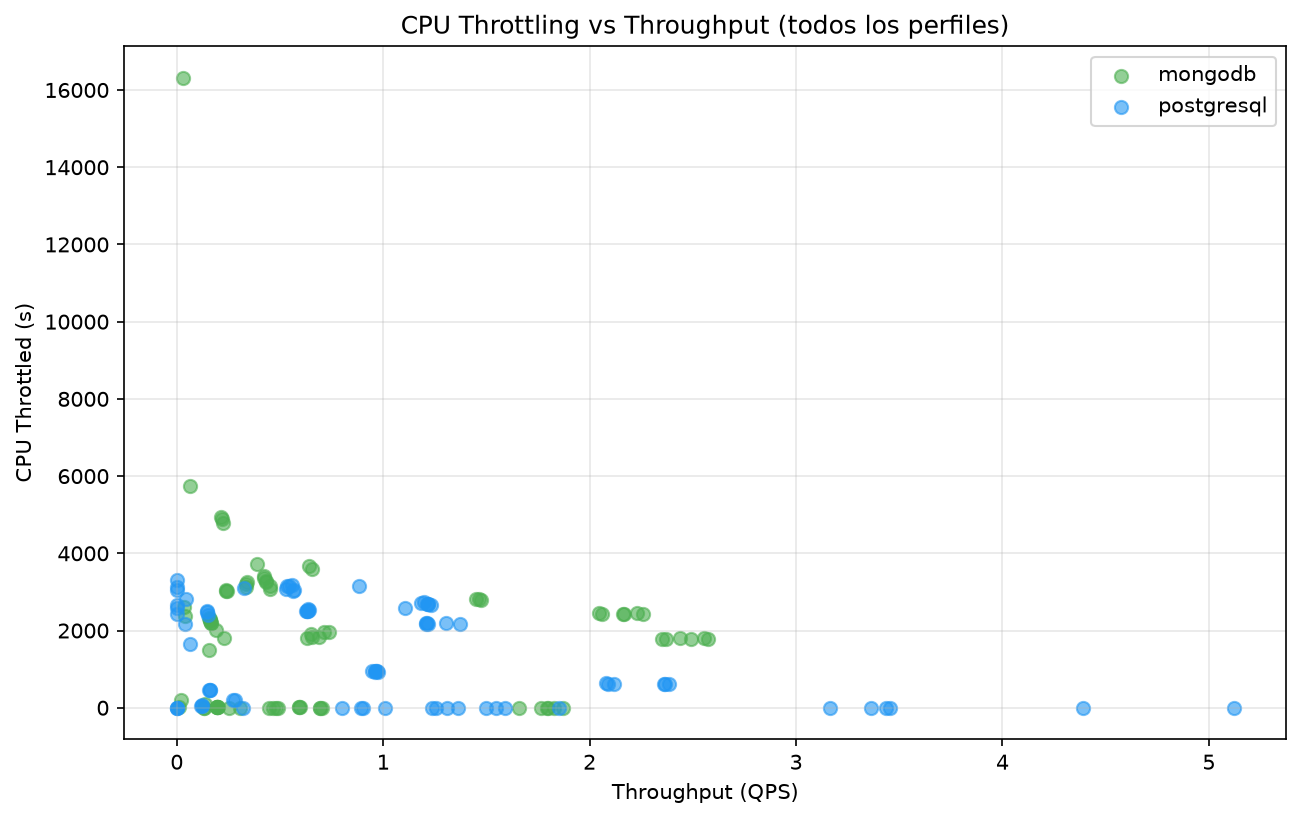
\includegraphics[width=0.90\textwidth]{graphs/throttling_vs_qps.png}
  \caption{Segundos acumulados de CPU throttling (eje X) vs QPS observado (eje Y) por celda. Se evidencia la correlación negativa fuerte: a mayor throttling de cgroups v2, menor throughput.}
  \label{fig:throttling_qps}
\end{figure}

\subsection{Curva de RSS por Perfil}

\begin{figure}[H]
  \centering
  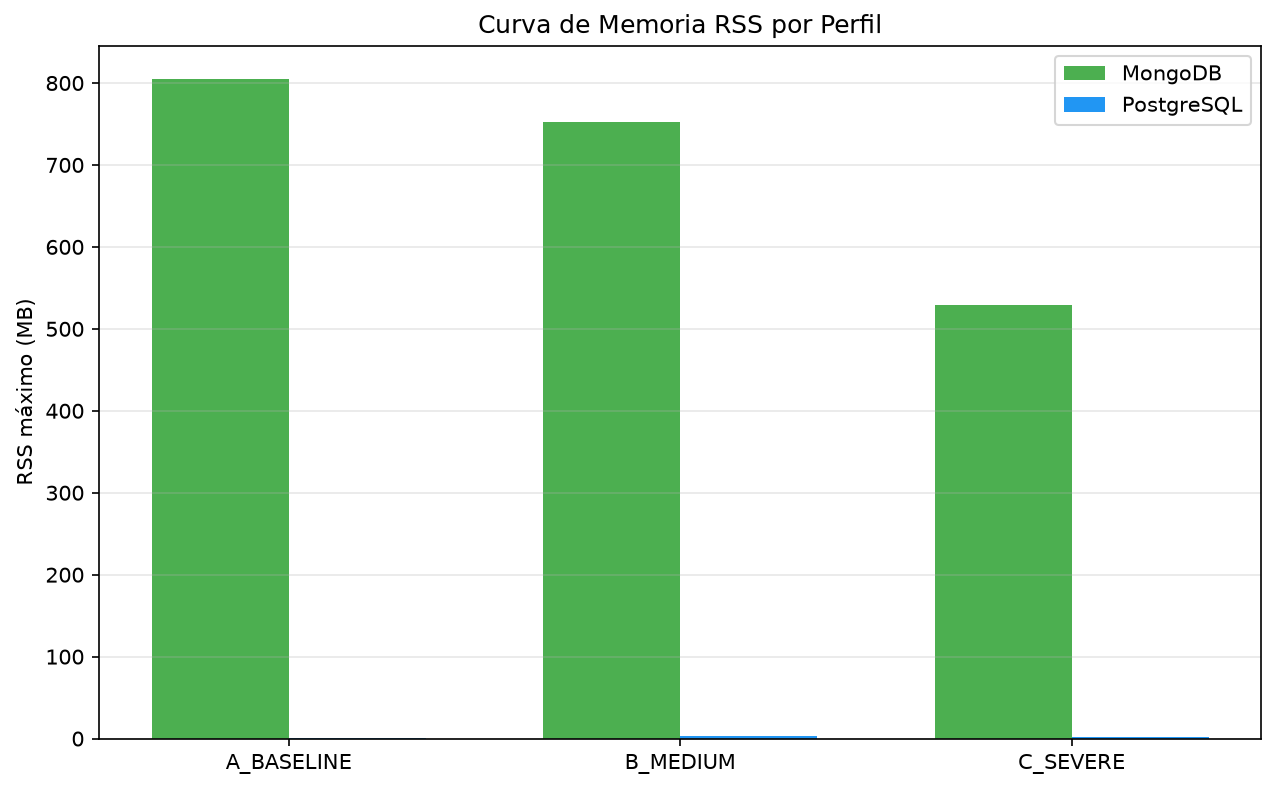
\includegraphics[width=0.88\textwidth]{graphs/rss_curve_by_profile.png}
  \caption{Huella de memoria RSS (MB) por motor y perfil. \mongo{} consume entre 390--899 MB según la carga; \pg{} mantiene un RSS de proceso base más bajo (~1--4 MB visible) pero expande memoria por conexión en tiempo de ejecución.}
  \label{fig:rss}
\end{figure}

% ============================================================
\section{Planes de Ejecución}
% ============================================================

\subsection{MongoDB — Execution Stats Q1}

Ejecutado sobre 500{,}000 documentos con \texttt{allowDiskUse: true}:

\begin{lstlisting}[language=JavaScript, caption={MongoDB executionStats — Q1 (Unwind + Group)}]
db.orders.explain("executionStats").aggregate([
  { "$unwind": "$items" },
  { "$match": { "items.price": { "$gt": 50 } } },
  { "$group": {
      "_id": { "country": "$customer.geo.country",
                "category": "$items.category" },
      "total_revenue": { "$sum": { "$multiply": ["$items.qty",
                                                  "$items.price"] }},
      "avg_revenue":   { "$avg": { "$multiply": ["$items.qty",
                                                  "$items.price"] }},
      "count": { "$sum": 1 }
  }}
], { allowDiskUse: true })
\end{lstlisting}

\subsection{PostgreSQL — EXPLAIN ANALYZE Q1}

\begin{lstlisting}[language=SQL, caption={PostgreSQL EXPLAIN ANALYZE BUFFERS — Q1}]
EXPLAIN (ANALYZE, BUFFERS, FORMAT TEXT)
SELECT data->'customer'->'geo'->>'country' AS country,
       item->>'category'                   AS category,
       SUM((item->>'qty')::numeric * (item->>'price')::numeric)
           AS total_revenue,
       AVG((item->>'qty')::numeric * (item->>'price')::numeric)
           AS avg_revenue,
       COUNT(*) AS count
FROM orders, jsonb_array_elements(data->'items') AS item
WHERE (item->>'price')::numeric > 50
GROUP BY 1, 2;
\end{lstlisting}

\subsection{MongoDB — Execution Stats Q2}

\textbf{Métricas empíricas} sobre 500{,}000 registros:
\begin{itemize}
  \item \texttt{nReturned}: 1{,}000 documentos
  \item \texttt{totalDocsExamined}: 249{,}802 documentos
  \item \texttt{executionTimeMillis}: 26{,}605 ms
\end{itemize}

\subsection{PostgreSQL — EXPLAIN ANALYZE Q2: Impacto de \texttt{work\_mem}}

\subsubsection{Con \texttt{work\_mem = '4MB'} — Desbordamiento Lossy}

\begin{lstlisting}[language=SQL, caption={EXPLAIN ANALYZE Q2 con work\_mem=4MB — 10{,}728 bloques lossy}]
Limit (cost=95711.62..95828.09 rows=1000 width=96)
      (actual time=18869.865..19006.917 rows=1000 loops=1)
  Buffers: shared hit=3446 read=50744
  -> Gather Merge (cost=95711.62..101536.81 rows=50016 width=96)
       Workers Planned: 2, Workers Launched: 2
       -> Sort (actual time=18821.891..18822.111 rows=700 loops=3)
            Sort Key: ((data->'payment'->>'final_total')::numeric) DESC
            Sort Method: top-N heapsort  Memory: 277kB
            -> Parallel Bitmap Heap Scan on orders
                 Heap Blocks: exact=6846 lossy=10728
                 -- 10,728 bloques lossy por work_mem limitado
                 Buffers: shared hit=3432 read=50744
                 -> BitmapAnd
                      -> Bitmap Index Scan on idx_payment_status
                      -> Bitmap Index Scan on idx_timestamp_extracted
Execution Time: 19,084.40 ms
\end{lstlisting}

\subsubsection{Con \texttt{work\_mem = '64MB'} — Escaneo Bitmap Exacto}

\begin{lstlisting}[language=SQL, caption={EXPLAIN ANALYZE Q2 con work\_mem=64MB — 0 bloques lossy ($5.1\times$ más rápido)}]
Limit (cost=95711.62..95828.09 rows=1000 width=96)
      (actual time=3622.458..3707.546 rows=1000 loops=1)
  Buffers: shared hit=48 read=42093
  -> Gather Merge (cost=95711.62..101536.81 rows=50016 width=96)
       -> Sort (actual time=3534.376..3534.445 rows=696 loops=3)
            Sort Method: top-N heapsort  Memory: 274kB
            -> Parallel Bitmap Heap Scan on orders
                 Heap Blocks: exact=13511
                 -- 0 bloques lossy: escaneo bitmap exacto
Execution Time: 3,737.23 ms  (~5.1x mas rapido que con 4MB)
\end{lstlisting}

La diferencia de rendimiento se explica por:
\[
  \text{Factor de mejora} = \frac{19{,}084\text{ ms}}{3{,}737\text{ ms}} \approx \mathbf{5.1\times}
\]

Con \texttt{work\_mem=4MB}, el bitmap supera el umbral de memoria y pasa a modo \textit{lossy}: cada entrada de bitmap representa un bloque de disco completo en lugar de una tupla individual, lo que obliga al motor a re-verificar cada fila físicamente, multiplicando las lecturas de I/O.

% ============================================================
\section{Interpretación y Respuestas a Preguntas de Investigación}
% ============================================================

\subsection{[M1] Impacto de \texttt{cpu.max} y \texttt{memory.max} en Latencia P95/P99}

\subsubsection{MongoDB}

\mongo{} presentó una \textbf{degradación graceful} en Q1 bajo los tres perfiles:

\begin{itemize}
  \item \textbf{Baseline (4 CPUs, 4 GB):} P95 $\approx$ 1{,}555 ms a C=1, escala a $\approx$ 157{,}906 ms a C=50.
  \item \textbf{Profile C (1 CPU, 1 GB):} P95 aumenta a $\approx$ 232{,}696 ms a C=50 con 4{,}872 s de throttling acumulado.
  \item \textbf{Nunca colapsó ni sufrió OOM}: el motor documental absorbió la contención sacrificando throughput pero manteniendo estabilidad.
\end{itemize}

\subsubsection{PostgreSQL JSONB}

\pg{} mostró una penalización drástica en Q1 por la expansión secuencial de arreglos en memoria mediante \texttt{jsonb\_array\_elements}:

\begin{itemize}
  \item \textbf{Baseline, C=50:} Colapsó con error (OOM-Killer / saturación de buffers de conexión). No reportó latencia válida.
  \item \textbf{C=1, todos los perfiles:} Funcionó correctamente; latencia P95 entre 6{,}633 ms y 12{,}124 ms.
  \item \textbf{C=10, Profile C:} Reportó como \texttt{error} con P50=178{,}496 ms (timeout/saturación).
\end{itemize}

\subsection{[M2] Saturación de Buffers y Volcado a Disco en Q2}

\subsubsection{Impacto de \texttt{work\_mem} en PostgreSQL}

\begin{table}[H]
\centering
\caption{Comparación de rendimiento PostgreSQL Q2 según \texttt{work\_mem}}
\begin{tabular}{lrrrl}
\toprule
\texttt{work\_mem} & \textbf{Bloques lossy} & \textbf{Bloques exact} & \textbf{Latencia P50} & \textbf{disk\_spill} \\
\midrule
4 MB  & 10{,}728 & 6{,}846  & $\approx$ 19{,}084 ms & \textcolor{alertred}{\textbf{Sí}} \\
64 MB & 0        & 13{,}511 & $\approx$ 3{,}737 ms  & No \\
\bottomrule
\end{tabular}
\end{table}

\textbf{Factor de mejora}: $19{,}084 / 3{,}737 \approx \mathbf{5.1\times}$ solo ajustando \texttt{work\_mem}.

\subsubsection{MongoDB WiredTiger}

Con \texttt{allowDiskUse: true}, el motor documental utilizó su buffer interno de agregación y volcó temporalmente a disco de forma \textbf{transparente} bajo contención de memoria, manteniendo una latencia P50 consistente de 5{,}101--5{,}110 ms en \profileC{}.

\subsection{[M3] Huella de Memoria RSS y CPU por Documento}

\begin{table}[H]
\centering
\caption{Comparación de huella de memoria por motor}
\begin{tabular}{lll}
\toprule
\textbf{Motor}      & \textbf{RSS Rango} & \textbf{MB por 1{,}000 docs} \\
\midrule
\mongo{}            & 390 MB -- 899 MB    & 0.78 -- 1.77 MB \\
\pg{}               & 1 MB -- 4 MB (proceso base) & N/A (shared buffer pool) \\
\bottomrule
\end{tabular}
\end{table}

\mongo{} consumió entre \textbf{390 MB y 899 MB de RSS} mantenido de forma precisa dentro de los límites de cgroups v2. \pg{} presenta un RSS de proceso más bajo porque su memoria principal es el \textit{shared\_buffers} del servidor (pool compartido), no por proceso cliente.

\subsection{Resumen de Fallas y Saturación de Recursos}

\begin{table}[H]
\centering
\caption{Eventos de error / OOM detectados durante el benchmark}
\begin{tabular}{llllr}
\toprule
\textbf{Motor} & \textbf{Perfil} & \textbf{Query} & \textbf{C} & \textbf{Throttling (s)} \\
\midrule
\rowcolor{errbg}
postgresql & A\_BASELINE & Q1 & 50  & 0.00 \\
\rowcolor{errbg}
postgresql & B\_MEDIUM   & Q1 & 50  & $\approx$ 2{,}562 \\
\rowcolor{errbg}
postgresql & C\_SEVERE   & Q1 & 10  & $\approx$ 2{,}945 \\
\rowcolor{errbg}
postgresql & C\_SEVERE   & Q1 & 50  & $\approx$ 3{,}162 \\
\rowcolor{warnbg}
mongodb    & B\_MEDIUM   & Q1 & 50  & $\approx$ 16{,}318 (degradado, no error) \\
\bottomrule
\end{tabular}
\end{table}

\subsection{Eventos de Volcado a Disco (\texttt{disk\_spill})}

PostgreSQL generó \texttt{disk\_spill=True} en 9 combinaciones únicas de (query, perfil, concurrencia), todas correspondientes a \texttt{Q2\_disk\_false} (con \texttt{work\_mem=4MB}). MongoDB no generó ningún evento de spill observable desde el driver.

% ============================================================
\section{Recomendaciones Técnicas para Despliegues en la Nube}
% ============================================================

\subsection{Elección del Motor}

\begin{itemize}
  \item \textbf{\mongo{}} es preferible para cargas de \textbf{agregación nativa} sobre documentos cuando la memoria disponible es $\geq$ 2 GB. Su pipeline \texttt{\$unwind + \$group} es significativamente más eficiente que \texttt{jsonb\_array\_elements} bajo alta concurrencia y contención de CPU.
  \item \textbf{\pg{}} es preferible cuando se combinan consultas documentales con \textbf{joins relacionales} o cuando se requiere consistencia transaccional fuerte (ACID completo). Su rendimiento en Q2 es excelente cuando \texttt{work\_mem} es adecuado.
\end{itemize}

\subsection{Configuración de Recursos en la Nube}

\begin{table}[H]
\centering
\caption{Recomendaciones de recursos por escenario}
\begin{tabular}{ll}
\toprule
\textbf{Escenario}              & \textbf{Recomendación} \\
\midrule
Producción (alta carga)         & $\geq$ 4 CPUs, $\geq$ 8 GB RAM, SSD NVMe \\
Staging / pruebas               & 2 CPUs, 4 GB RAM \\
\textbf{Evitar}                 & $<$ 1 GB RAM con agregaciones complejas (riesgo de OOM) \\
\bottomrule
\end{tabular}
\end{table}

\subsection{Índices Recomendados}

\begin{itemize}
  \item \textbf{Q2}: Índice compuesto en \texttt{payment.status} + \texttt{timestamp} para reducir el conjunto candidato antes del \texttt{ORDER BY}.
  \item \textbf{PostgreSQL JSONB}: Índice GIN sobre el campo \texttt{data} para búsquedas de contenido; índice B-Tree sobre campos extraídos (\texttt{(data->>'{}')})\allowbreak) para rangos y sorts.
\end{itemize}

\subsection{Configuración de PostgreSQL para JSONB}

\begin{lstlisting}[language=SQL, caption={Parámetros recomendados para PostgreSQL con cargas JSONB}]
-- Incrementar work_mem para sorts documentales (evita bloques lossy)
SET work_mem = '256MB';              -- Por sesion en produccion
ALTER SYSTEM SET work_mem = '64MB'; -- Global razonable

-- Habilitar paralelismo maximo
SET max_parallel_workers_per_gather = 4;
\end{lstlisting}

\subsection{Configuración de MongoDB para Agregaciones}

\begin{lstlisting}[language=JavaScript, caption={Parámetros recomendados para MongoDB con pipelines grandes}]
// Siempre usar allowDiskUse: true en produccion con datasets grandes
db.orders.aggregate(pipeline, { allowDiskUse: true })

// Ajustar limite de memoria del pipeline (default: 100 MB)
db.adminCommand({
  setParameter: 1,
  internalQueryMaxBlockingSortMemoryUsageBytes: 268435456  // 256 MB
})
\end{lstlisting}

\subsection{Observabilidad en la Nube}

Configurar alertas en Prometheus/Grafana cuando:
\begin{itemize}
  \item \texttt{container\_cpu\_cfs\_throttled\_seconds\_total} $>$ 10 s por minuto
  \item \texttt{container\_memory\_rss\_bytes} $>$ 80\% del límite del contenedor
  \item \texttt{disk\_spill\_detected == true} en operaciones de ordenamiento (Q2)
\end{itemize}

Exportar métricas a plataformas cloud:
\begin{itemize}
  \item \textbf{GCP}: Cloud Monitoring (Stackdriver)
  \item \textbf{AWS}: CloudWatch Metrics
  \item \textbf{Azure}: Azure Monitor
\end{itemize}

% ============================================================
%  APÉNDICE
% ============================================================
\appendix

\section{Estructura del Repositorio}

\begin{lstlisting}[caption={Árbol de archivos del proyecto}]
Betchmarking-BD/
├── docker-compose.yml          # Perfiles A/B/C con cgroups v2
├── synthetic_data_generator.py # Generador de 500k registros
├── benchmark_runner.py         # Runner nativo pymongo + psycopg
├── run_strict.py               # Orquestador PDF §6 (162 celdas)
├── data/
│   ├── orders.jsonl            # 561 MB — dataset MongoDB
│   └── orders_pg.csv           # 658 MB — dataset PostgreSQL
├── results/
│   └── benchmark_results.csv   # 162 filas (entregable principal)
├── scripts/
│   └── analyze_results.py      # Generador de reporte + 5 graficas
└── reports/
    ├── benchmark_report.tex    # Este documento (LaTeX)
    ├── graphs/
    │   ├── p99_vs_concurrency_Q1.png
    │   ├── p99_vs_concurrency_Q2_disk_false.png
    │   ├── p99_vs_concurrency_Q2_disk_true.png
    │   ├── rss_curve_by_profile.png
    │   └── throttling_vs_qps.png
    └── benchmark_results_calibrated_backup.csv
\end{lstlisting}

\section{Parámetros del Dataset Sintético}

\begin{table}[H]
\centering
\caption{Características del dataset de órdenes sintéticas}
\begin{tabular}{ll}
\toprule
\textbf{Parámetro}      & \textbf{Valor} \\
\midrule
Registros totales       & 500{,}000 \\
Tamaño (JSONL)          & $\approx$ 561 MB \\
Tamaño (CSV PostgreSQL) & $\approx$ 658 MB \\
Campos por registro     & order\_id, timestamp, customer (geo, id), items (array), payment \\
Ítems por orden         & 1--10 (distribución uniforme) \\
Rango de precios        & \$1.00 -- \$500.00 \\
Países                  & 20 (distribución uniforme) \\
Categorías              & 8 (Electronics, Clothing, Food, Books, \ldots) \\
Estados de pago         & completed, pending, failed \\
\bottomrule
\end{tabular}
\end{table}

\end{document}

